\documentclass[titlepage,a4paper,11pt]{article}
\usepackage{graphicx} % Required for inserting images
\usepackage{float}
\usepackage{url}
\usepackage{booktabs}
\usepackage{geometry}
\usepackage{ragged2e}
\usepackage[svgnames]{xcolor}
\usepackage{makecell, tabularx}
    \setcellgapes{2pt}
    \makeatletter
    \newcommand*{\compress}{\@minipagetrue}
    \makeatother
    \newcolumntype{I}{ >{\RaggedRight\compress\itemize}X<{\enditemize}}
    \newcommand*{\mcl}[1]{\multicolumn{1}{l|}{#1}}
\usepackage[skip=1ex]{caption}
\usepackage{enumitem}\usepackage{tabularx}
\usepackage[utf8]{inputenc}
\usepackage[T1]{fontenc}

\begin{document}

\begin{titlepage}
\begin{center}
  \bfseries
  \huge UNIVERSITY OF SOUTHERN DENMARK
  \vskip.2in
  \textsc{\LARGE Faculty of engineering}
  \vskip.2in
  \large BEng Mechatronics
  \vskip1in
  \Large Mechatronics Semester Project 4
  \vskip1.5in
  \emph{\huge Ladybug}
\end{center}

\vskip1.4in

\begin{minipage}{.35\textwidth}
  \begin{flushleft}
    \bfseries\large Supervisor:\par \emph{Lars Duggen} \par \emph{Davi Goncalves Accioli} \end{flushleft}
\end{minipage}
\hskip.4\textwidth
\begin{minipage}{.4\textwidth}
  \begin{flushleft}
    \bfseries\large Group: 7 \par \emph{Tobias Blaabjerg Karlsen} \par \emph{Artis Fils} \par \emph{Thor Uerkvitz} \par \emph{Choyon Mainul Hasan} \par \emph{Johan Paul} \par \emph{Ruta Miglava}
  \end{flushleft}
\end{minipage}

\vfill
\centering
\bfseries
\Large Year \the\year
\end{titlepage}

\section{Background}

Possessing the ability of flight and minimising effort and casualties has always been desirable for the utility flight can provide.
The first unmanned aircrafts can be dated back to 1849, where Austria seemingly had utilised unmanned air balloons with stuffed explosives to attack Venice. \cite{Vyas2020}
Ever since an unmanned aircraft vehicle (UAV), is one that is flown by technological means or as a pre-programmed flight without pilot control, as defined by the ECAA Transport Agency \cite{Droner}, nowadays called drones, have risen in popularity.


Because of this, UAVs come in a wide range of sizes and weights.
UAVs often include multirotor, radio-controlled miniature helicopters, and aeroplanes \cite{Ann2012}.
As a result, there are several methods to categorize drones. The performance parameters of UAVs, such as weight, wingspan, wing load, flight range, maximum flying altitude, speed, and production cost, are typically used to categorize them \cite{Hassanalian2017}.
According to how the lift is produced, drones may also be divided into fixed-wing and rotating-wing types.
According to the drone code category, the European Aviation Safety Agency (EASA) categorizes unmanned aircraft by weight.
The EASA regulations for open categories, or drones without an EASA class designation, are summarized succinctly and simply in Figure~\ref{fig:Table} \cite{Euasa}.

Self-built drones weighing up to 250 g, as described in Figure~\ref{fig:Table}, may be used without registration if the drone is a toy or the drone is not equipped with a camera, the remaining drones must be registered, and the pilot must pass examinations \cite{Euasa}. In this paper, self-built rotary drones with four wings or propellers are the objective, making weight-based classification suitable.

\begin{figure}[H]
    \centering
    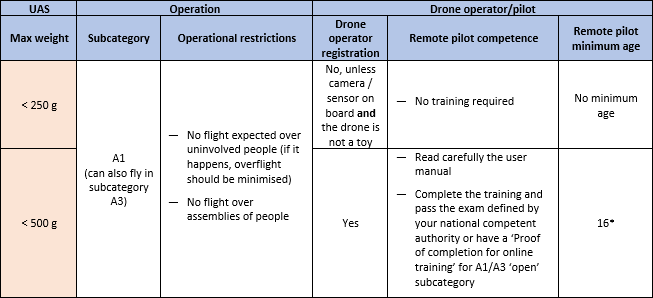
\includegraphics[scale = 0.9]{classification.PNG}
    \caption{Classification and restrictions for non-EASA class drones \cite{Euasa}}
    \label{fig:Table}
\end{figure}


When it comes to the state-of-the-art project, PULP-DroNet is a deep learning-powered visual navigation engine that enables autonomous navigation of a pocket-size quadrotor in a previously unseen environment. Thanks to PULP-DroNet the nano-drone can explore the environment, avoiding collisions also with dynamic obstacles, in complete autonomy -- no human operator, no ad-hoc external signals, and no remote laptop! This means that all the complex computations are done directly aboard the vehicle and very fast. The visual navigation engine is composed of both a software and a hardware part. \cite{Niculescu2021}

When it comes to the future, the simulated pollination of agricultural plants by means of nano copter can provide collecting and delivering pollen in the mode of automatic control. A design of nano copter for pollination can be made on the basis of innovative modification of existing model by its reprogramming with regard to its flight controller that is to be fully adapted to computer interface. The robotic system is offered specially for artificial pollination in conditions of greenhouses and minor agricultural enterprises. \cite{Abutalipov2016}


\section{Problem statement}

The utility of smaller drones are immense, where it can be used in surveillance, toys and potentially to also be part of a swarm of drones. Although, there are smaller drones existing in the current market, we would like to challenge ourselves to build one ourselves, where certain goals ranging from functionality to budget are listed below.


\subsection{Primary goals }
\begin{itemize}
    \item
          Net maximum weight of the drone is 250 grams. Weight under 250 grams ensures it falls under A1 category in EU regulations. 1
    \item
          Flight time of 20 seconds.
    \item
          Stress of the structural system should not exceed rupture point. System does not experience fracture.
\end{itemize}


\subsection{Secondary goals}
\begin{itemize}
    \item
          Flight time of minimum one minute.
    \item
          Can land with acceleration less than 9.8 m/s2.
    \item
          Stress of the drone system should not exceed the yield point. System does not experience plastic deformation.
    \item
          Drone is remote controllable.
    \item
          Drone can fly in formation with another identical drone.
    \item
          Total production cost of the drone is under 500 DKK (Not including remote controller).
    \item
          Drone can play audio.
\end{itemize}



\subsection{Constraints}

\begin{itemize}
    \item
          Budget for entirety of project is 2000 DKK.
    \item
          Time available to finish the project is 4 months.
    \item
          Drone should have a minimum hover time of 5 seconds.
    \item
          Drone should be fully functional and able to take off again after landing.
    \item
          No use of flight controller software or unmanned vehicle Autopilot software Suite, capable of controlling autonomous vehicles.
\end{itemize}


\section {Test Specifications}
\subsection{Primary goals:}
\begin{itemize}
    \item
          To test this, the drone will be weighed with a scale of a precision on 0,1 grams.
    \item
          In order to test the flight time, a stopwatch will be started from the moment the drone leaves the ground and is stopped as soon as it lands.
    \item
          This goal will be the tested trough FEM, ensuring that the chosen material for the drones body, will not rupture.
\end{itemize}

\subsection{Secondary goals}
\begin{itemize}
    \item
          This will be tested with the same method as primary goals tests point 2.
    \item
          This will be tested with a mobile phone, recording the drones landing, using the drones position compared to the timestamp of the video.
    \item
          This will be tested with the same goals as primary goals test point 3.
    \item
          This will be tested by the possibility of sending wireless signals to the drone, with the drone reacting to those send signals.
    \item
          This will be tested purely by ear, listening to the drones output.
    \item
          This will be tested by mobile phone video, looking at the drones positions at given timestamps.
    \item
          This will be tested trough summing the price for each single part, ensuring that it doesn’t exceed 500 DKK.
\end{itemize}

\subsection{Constraints}
\begin{itemize}
    \item
          This will be done with the same method as the secondary goals test, though ensuring the project cost is over 2000 DKK.
    \item
          To evaluate the time constraint point of the project, the goal fullfilments will be evaluated in the end of the project period. In the case that all primary goals are fulfilled, the constraint is succeeded.
    \item
          This will be tested with a stopwatch, ensuring that the hover time is atleast 5 seconds.
    \item
          This will be tested with making the drone take off right after a landing, making sure that the drone is fully operational at the second take-off.
    \item
          This will fulfilled by not employing any of the aforementioned in the drone.
\end{itemize}

\section{Prototyping}
\subsection{Embedded development environment}

Software shoud take care of the motor control, IMU output readings and remote control, this could create complications, as essentially they would interrupt each other. A way of multitasking should be introduced.
"An RTOS (Real-Time Operating System) is a software component that lets you rapidly switch between different running sections of your code. Think of it as having several loop() functions in an Arduino sketch where they all run at the same time." \cite{Joe2019}

After research, the list was narrowed to two top condenders – FreeRTOS and Zephyr. Both solutions are open source, widely used and support the Microcontroller board we have chosen. \cite{Lemberg}
According to 2018 IoT Developer Survey \cite{IOT}, FreeRTOS is one of the most popular OS used and while Zephyr only received a 2.8 \% rating in 2018, it is often described as one of the fastest growing RTOS and in 2022 has become the largest open-source RTOS project by the number of commits and developers. (See Figure~\ref{fig:iot_os})
\begin{figure}[H]
    \centering
    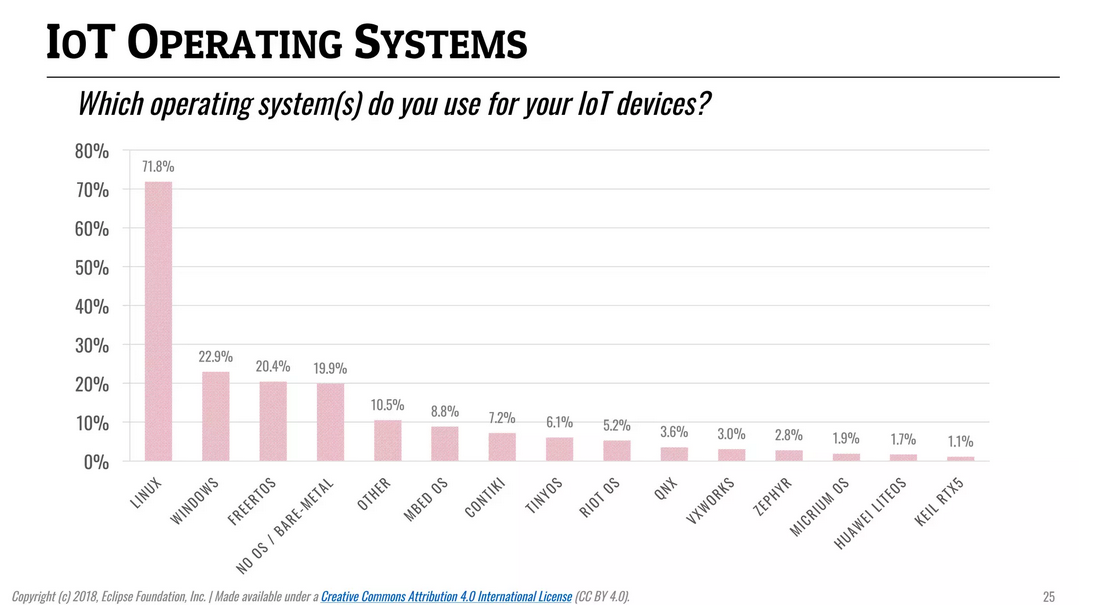
\includegraphics[scale = 0.5]{iot_os.PNG}
    \caption{IoT Developer Survey 2018 results}
    \label{fig:iot_os}
\end{figure}

To decide between the RTOS choice, a pros and cons table was created and evaluated. \cite{Comparison} (See Table~\ref{table.rtos})

\begin{table}[H]
      \makegapedcells
  \setlist[itemize]{font=\color{black},
                    nosep,
                    leftmargin=*,
                    after=\vspace*{-\baselineskip}}
      \setlength{\tabcolsep}{3pt}
  \begin{tabularx}{\linewidth}{|>{\RaggedRight}p{25mm}|*{2}{I |}}
      \hline
  RTOS
      &   \mcl{Advantages}    &   \mcl{Disadvantages}        \\
      \hline
  FreeRTOS 
      &   \item Suitable for begginers
          \item Open source – online comunity support available 
          \item Libraries for Seeed XIAO Sense available
          \item Constantly improved
          \item Fast code execution
          \item Low memory consuption
          &   \item Not event-driven (scheduler will only be called once in a certain period of time)
              \item Less flexible
              \\
      \hline
  ZephyrRTOS
      &   \item Open source – online comunity support available
          \item Libraries for Seeed XIAO Sense available
          \item Constantly improved
          \item Designed to ensure energy efficiency
          \item Highly configurable
          \item Event-driven
          \item Kernel can create additional system threads
          \item Possible to exclude multithreading
          \item Additional debugging features
          \item Supported by Nordic Semiconductor
          &   \item More difficult to set-up
              \item Potentially complicated to use with no experience
              \\
      \hline

\end{tabularx}
\caption{Comparison between ZephyrRTOS and FreeRTOS}
\label{table.rtos}
\end{table}

It was evaluated, that overall FreeRTOS seems to be a better established more simple solution to be used in case of no experience, whereas Zephyr offers more flexibility and is a fast growing popular solution well suited for our application and would be a worthwile investment to build our skillset for future projects. \cite{Industry}

As the Seeeduino XIAO nRF52840 Sense, uses the nRF52840 microcontroler, so looking to Nordic Semiconductor nRF Connect SDK for development, which uses a RTOS called ZephyrRTOS.
Additionally, the SDK provides useful tools for development, such as build, flashing and debugging actions. \cite{nRF}


Seeed XIAO nRF52840 is not natively suported on on nRF Connect SDK, but as ZephyrRTOS supports it. \cite{docsZephyr}

There is a caviat around this, we can fetch profiles from GitHub of the current version of Zephyr via \path{Zephyr/boards/arm/xiao_ble} at main branch \cite{gitZephyr} and import the needed files into the SDK version of Zephyr we have.
In our case the path of the files would be in \path{~\ncs\v2.3.0-rc1\zephyr\boards\arm} .
After doing so, following the steps in the DevAcademy, nRF Connect SDK Fundamentals, Lesson 1 can be followed for setup. Then a blinky application can be created, and built via nRF Connect.
After a build of the application is created, a files for flashing will be created in the "build" subdirectory of the application.
To flash the Seeed XIAO nRF52840 Sense chip, entering a bootloader is needed, as it ships with the Adafruit nRF52 Bootloader, which supports UF2 flashing. \cite{docsZephyr}
Further more, a zephyr.ut2 file can be found in the "build" subdirectory of the application, after building the application, as we have done.
To access the bootloader, connect the Seeed XIAO to a PC.
Now to enter and flash an application, the reset button on the Seeed board should be clicked two times in quick succession, this will propmt the memory of the Seeed board on your PC.
Now find the previously mentioned zephyr.ut2 and drag it in to the memory of the Seeed board, and this will flash the board with the new application.

A issue accured when trying to test the "Hello World" application, when connecting to serial monitor no output is given.
After further investigation, it was noticed that the Seeed documentation, mentiones no debugging interface, hence no USB serial exists.
To solve the issue, an application called "console", from \path{zephyr/samples/subsys/usb/console} was cloned, in order to test a virtual USB serial connection, with the use of CDC ACM UART. \cite{gitZephyr}
After building and flashing, results were achieved. (See Figure~\ref{fig:serial})

\begin{figure}[H]
    \centering
    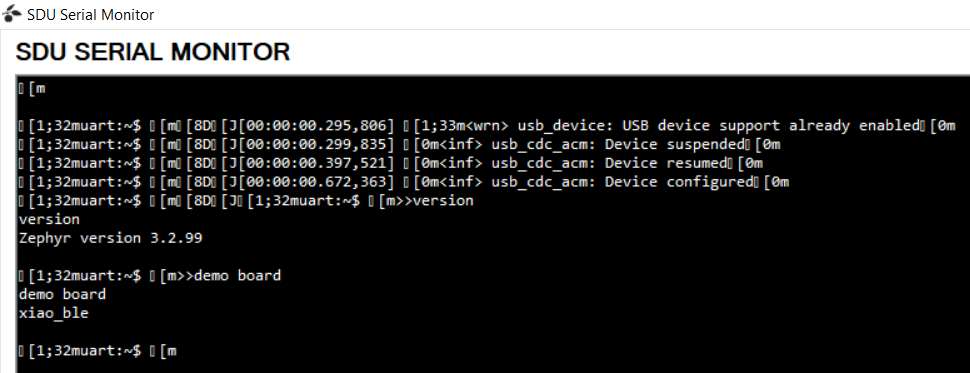
\includegraphics[scale = 0.7]{serial_monitor.png}
    \caption{Serial output of the XIAO MCU}
    \label{fig:serial}
\end{figure}

Another issue that arose was debugging. The Seeed XIAO nRF52840 Sense does not have any sort of built in debugging tools. \cite{wikiSeeed}
One can use a J-link debugging tool, but a caviet was found, which was GDB stub, which Zephyr supports, this would save budget. \cite{docsZephyr}

After achieving a succesful development cycle, it was conducted, that the use of ZephyrRTOS is possible with our current setup.
After further consultation with the supervisors, it was conducted, that the writers of the project have no skills in RTOS, more specifically in threading, and with the guidence of Davi, it was concluded, that acquiring such skills would be outside the scope of the project, as the main focus is control engineering.

\pagebreak
\bibliographystyle{plain}
\bibliography{references}
\appendix

\end{document}
